\section{The complete survivable embedded virtual network algorithm}
In this section, we first present that design procedure of augmented resource allocation  of SeVN graph, we also give out resource demand allocation method fitting for both FD-SeVN and FI-SeVN embedding, since the difference between FD-SeVN and FI-SeVN in embedding approach could be reconciled by a general resources sharing constraint. More details would be elaborated in the following part.

Besides, with respect to the node embedding even and virtual links embedding, because not all the virtual links or not all their bandwidth would be employed simultaneously under single node failure, some virtual links could share substrate resources if they are embedded on the same substrate link, which would reduce the total substrate bandwidth needed.


\subsection{Embed Augmented Backup Resource}
From Sec.\ref{lab:DynamicProgrammingEquation}, we have obtained map relationship with respect to node $v_i$ failure, then compute out that every node should to be reallocated how much computation and every link should to be reallocated how much bandwidth in substrate network SN as shown in Fig.\ref{fig:AugmentResource}. As most virtual network embedding algorithm, node mapping phase had been completed with respect to our algorithm, the next procedure give out edge mapping phase. we use standard shortest path algorithm, dijkstra algorithm, for requesting path of substrate node with respect to every virtual network's node, then reallocate some bandwidth to this path of substrate network for this virtual network survivable request.

\begin{figure}
  \centering
  % Requires \usepackage{graphicx}
  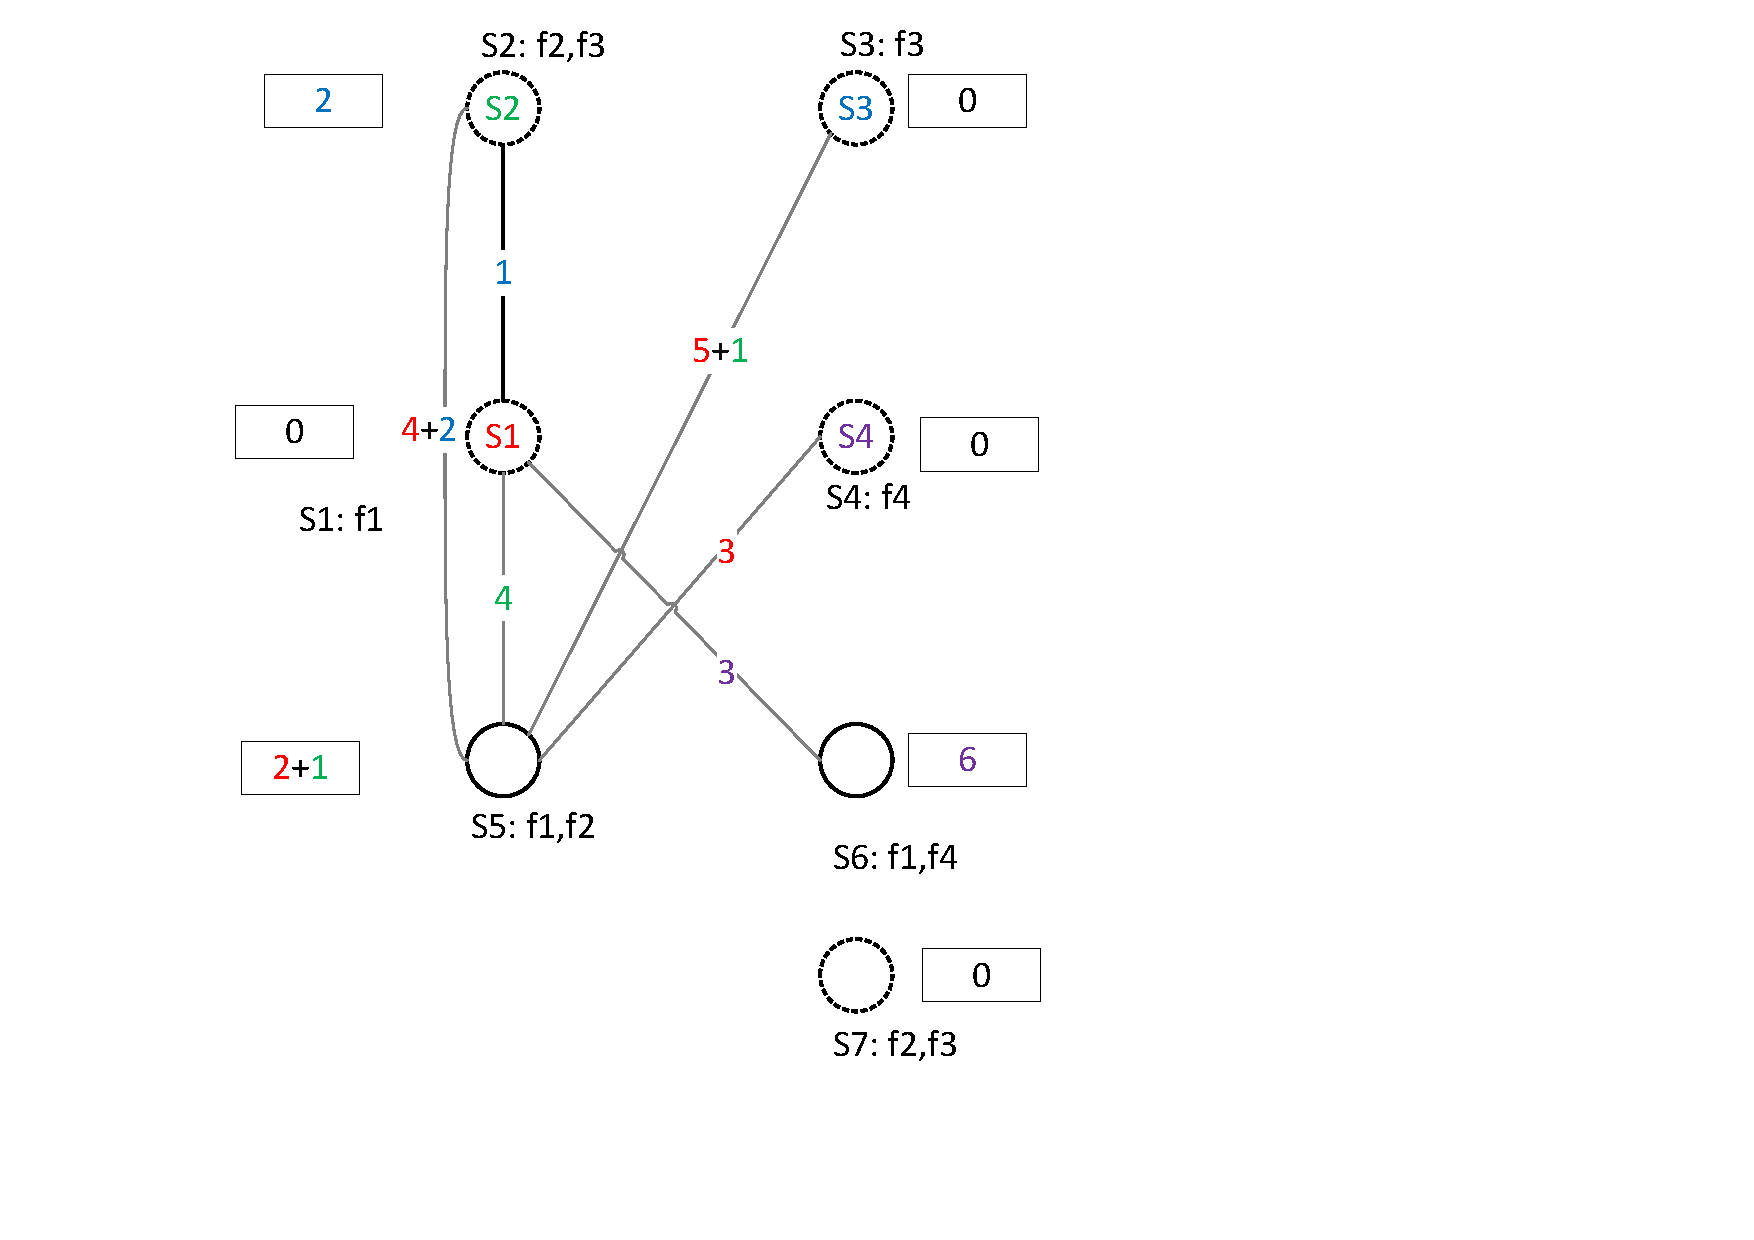
\includegraphics[width=2in]{Fig/AugmentResource}\\
  \caption{Augmented Resource}\label{fig:AugmentResource}
\end{figure}

Finally, we repeat the procedure of graph decomposition and multiple knapsack problem for each following node failure to construct the graph of final FD-SeVN. As shown in Fig.\ref{fig:FD}, partial augmented resource which is labeled consecutively with different color of the SeVN for each node failure is presented. It is worth noting that, every step of partial augmented resource is based on the previous step.

\subsection{Algorithm procedure}
In this section, we describe complete our algorithm $\MyAlgorithmMethodAbrreviation$ procedure of SeVN problem in Alg.\ref{alg:SeVNAlg}
\begin{algorithm}
\label{alg:SeVNAlg}
\caption{survivable embedded virtual network request algorithm}
\begin{algorithmic}[1]
\REQUIRE $G^V (V^V,E^V,f^V,C^V,B^V)$:  topological graph of virtual network's request; $G^S (V^S,E^S,F^S,C^S,B^S)$, topological graph of substrate network .
\ENSURE generate SeVN and embed SeVN augment resource into substrate network.
\STATE embed VN $G^V$ into substrate network $G^S$.
\STATE extract embedded virtual network eVN $G^*$ from SN corresponding to this VN embedding request
%\STATE AllMinimumCycle($G(V,E)$)
\FORALL{$v_i$ such that $v_i\in$ virtual node}
\STATE decompose eVN into two star structure sets $STAR^L$ and $STAR^R$ from graph $G^*$.
\STATE construct items based star structure set $STAR^L$.
\STATE construct knapsacks based star structure set $STAR^R$ from embedded virtual network eVN.
\STATE construct alignment cost matrix based graph edit distance method\cite{sanfeliu1983distance}
\STATE solve multiple knapsack problem through dynamic programming.
\STATE add new nodes ,connect new edge, allocate node computing and edge's bandwidth into $G^*$ to construct new graph $G^*$.
\ENDFOR
\STATE embed new additional(augment) boot up resource or startup new node from SeVN $G^*$ into substrate network $G^S$
\RETURN SeVN,$G^S$
\end{algorithmic}
\end{algorithm}

1 node+2 node computaion+12 bandwidth
0 node+1 node computaion+5 bandwidth
1 node+5 node computaion+11 bandwidth
1 node+6 node computaion+3 bandwidth
=3 node+14 node computaion+31 bandwidth

1 node+2 node computaion+12 bandwidth
0 node+1 node computaion+5 bandwidth
0 node+2 node computaion+3 bandwidth
1 node+6 node computaion+3 bandwidth
=2 node+11 node computaion+23 bandwidth
